\documentclass[
  digital, %% Replace with `printed` to enable the default options for the printed version
  oneside,
  notable, %% `table` causes the coloring of tables. Replace with `notable` to restore plain tables.
  nolof,     %% `lof` prints the List of Figures. Replace with `nolof` to hide the List of Figures.
  nolot     %% `lot` rints the List of Tables. Replace with `nolot` to hide the List of Tables.
  %% More options are listed in the user guide at
  %% <http://mirrors.ctan.org/macros/latex/contrib/fithesis/guide/mu/fi.pdf>.
]{fithesis3}
\usepackage[utf8]{inputenc}
\usepackage{textcomp}
\usepackage{color}
\usepackage[hyphens]{url}
\usepackage{multirow}
\usepackage{seqsplit}

%% The following section sets up the locales used in the thesis.
%\usepackage[resetfonts]{cmap} %% We need to load the T2A font encoding
%\usepackage[T1,T2A]{fontenc}  %% to use the Cyrillic fonts with Russian texts.



\thesissetup{
    date          = 2017/05/22,
    university    = mu,
    faculty       = fi,
    type          = mgr,
    author        = {Josef Pavelec},
    gender        = m,
    advisor       = {RNDr. Andriy Stetsko, PhD.},
    title         = {Optimization of JVM settings for application performance},
    keywords      = {JVM settings, Optimization},
%%    TeXkeywords   = {keyword1, keyword2, \ldots},
}
\thesislong{abstract}{
    Will be written in the end.
}
\thesislong{thanks}{
    Will be written in the end.
}



%%% ======================================================= %%%

\begin{document}
\chapter{Introduction}
    Will be written in the end.

%%% ======================================================= %%%
\chapter{Java Virtual Machine}

Java Virtual Machine (JVM) is an abstract computing machine. JVM can not process any program written in Java language (stored in \texttt{java} source file) but it executes only the program called \textit{bytecode} which is stored in a \texttt{class} file. A Java \texttt{class} file is produced from \texttt{java} source file by Java compiler (\texttt{javac program.java} command). JVM, like a real computing machine, has its own instruction set for processing \textit{bytecode}. For running compiled Java program, it's necessary to have only an implementation of JVM for a given platform. Described approach offers the ability for applications to be developed in a platform-independent manner, and it can be shortened by Sun Microsystems slogan: "\textit{Write once, run anywhere}". \cite{spec}

In the context of the JVM it should distinguish three terms:
\begin{itemize}
	\item "\textbf{specification} is a document that formally describes what is required of a JVM implementation.
	\item \textbf{implementation} is a computer program that meets the requirements of the JVM specification.
	\item \textbf{instance} is an implementation running in a process that executes a computer program compiled into Java bytecode." \cite{brief}
\end{itemize}

For the correct implementation of Java Virtual Machine you only need to be able to read \texttt{class} file and perform the specified operations. The Java Virtual Machine specification doesn't contains any requirements or constraints for implementation of JVM. For this reason, the memory layout of run-time data areas, the garbage-collection algorithm used, any internal optimization of the JVM instruction (e.g. translating them into native code) and other matters connected with implementation of JVM are left to the implementor. Consequently, the JVM specification doesn't describe the possible ways how to adjust a JVM behaviour to achieve a better performance of a running application. \cite{spec}

There are many implementations of JVM\footnote{An extensive list of JVM implementation is accessible on \url{https://en.wikipedia.org/wiki/List_of_Java_virtual_machines}}. This chapter of the thesis deals with the Java HotSpot Virtual Machine respective to Java Development Kit 8 (JDK 8) which is the primary reference JVM implementation. This version is the latest because JDK 9 release is scheduled for July 2017\footnote{\url{https://blogs.oracle.com/java/proposed-schedule-change-for-java-9}}.

\section{Java HotSpot VM}
The Java 8 HotSpot Virtual Machine implementation is maintained by Oracle corporation. It implements JVM 8 specification and seeks to achieve best results for executing \textit{bytecode} in areas such as automatic memory management or compilation to native code.

Since the first version of JVM was interpreted, the statement "\textit{Java is slow}" has persisted notwithstanding it's not true in these days. More information regarding this topic will be provided in next sections.

As mentioned earlier, the main purpose of JVM is executing \textit{bytecode} on a specific platform which means translating \textit{bytecode} to native code of CPU. Since interpreting of \textit{bytecode} had appeared inefficient, an approach called \textit{Just-In-Time} compilation (JIT) was introduced in Java 1.2 \cite{javavsc}. A JVM implementation with JIT compiler translates a program into native code on the fly. Native code is cached and reused without recompiled. The extent of native code optimization is limited in this case because translation should be fast.

Java HotSpot VM is appropriately named after approach it takes toward compiling the code. A small part of the code is executed frequently in common programs. Frequent code sections represent approximately 20 \%\footnote{\url{http://artiomg.blogspot.cz/2011/10/just-in-time-compiler-jit-in-hotspot.html}} which are in accordance with the Pareto principle. These sections are called \textit{hot spots}. The more the section of code is executed, the hotter section is said to be. The faster will be \textit{hot spots} executed, the higher performance of an application will be. \cite{scott}

Oracle's HotSpot VM combines interpretation and translation. First, it interprets all code and concurrently collects information how often code is executed and additional data. After that JVM uses collected information for compilation with a high level of optimization. The more information about code JVM has, the more level of optimization it can achieve but for the price of the slow interpretation in the beginning. Actually, depending on the aggressiveness and level of optimization there are two different compilers in HotSpot JVM -- \textbf{client} and \textbf{server} (see sections \ref{clientcomp} and \ref{servercomp}).

The choice of which compiler to use is often the only one decision that is done during the compiler tuning. Even, choosing of compiler must be considered before JVM is installed because different JVM binaries contain different compilers. \cite{scott}

Another important role of any JVM implementations is automatic memory management known as \textbf{Garbage collections (GC)}. There are four different algorithms (called as Garbage Collectors) that provide this task in HotSpot:
\begin{itemize}
	\item \textbf{serial collector}
	\item \textbf{parallel (throughput) collector}
	\item \textbf{concurrent (CMS) collector}
	\item \textbf{G1 collector}
\end{itemize}
Every of garbage collectors has quite a different performance characteristics and is suitable for a different category of an application and environment. \cite{scott}

\subsection{Client compiler}\label{clientcomp}
The HotSpot VM's client compiler is designed for faster application startup, quick compilation and smaller memory footprint. This type of compiler is typically suitable for GUI application because there is a responsiveness without jitter desired. \cite{hunt}

The name \textit{client} compiler comes from the command-line argument \texttt{-client} used to select the compiler. When 64-bit version of the JDK is used, this option is ignored and \textit{server} compiler (see section \ref{servercomp}) will be used. Sometimes client compiler is called \textit{compiler 1} or shortly \textit{C1}\footnote{The short notation is used in list of advanced options. See section \ref{secoptions}}. \cite{scott} \cite{java}
\subsection{Server compiler}\label{servercomp}
The second HotSpot VM's compiler targets high throughput and peak performance. The server compiler uses the most powerful optimizations it can. The disadvantage of this behaviour is a fact, that time for getting an essential information for top optimization can be long. Concurrently, the overall memory footprint of server compiler is larger due to more data to handle. Native code produced by server compiler will be definitely more effective. Therefore advantages of high optimization of code depend on a run time of an application and the server compiler is suitable for long running applications. \cite{hunt}

The \texttt{-server} option serves fo use the server compiler. The server compiler is also marked as \textit{compiler 2} or \textit{C2}.

A technique called \textit{tiered compilation} combines a client compiler fast startup and a server compiler high optimization. With the tiered compilation, the code is first compiled by the client compiler, as it becomes hot, it is recompiled by the server compiler. The tiered compilation is available only for server compiler\footnote{If command \texttt{java -client -XX:+TieredCompilation}\textit{ programName} is used, \texttt{-XX:+TieredCompilation} option is quietly turned off. \cite{scott}}. The tiered compilation was introduced in the JDK 7 and it becomes as default in the JDK 8. \cite{scott}
\subsection{Garbage collectors}

\section{Setting options}\label{secoptions}
There are many options how to adjust behaviour JVM. For example, we may enforce to use parallel collector or set maximum heap\footnote{Heap is a memory area that JVM uses for residing the Java objects.} size. Options are divided into several categories:
\begin{itemize}
	\item "\textbf{Standard options} -- are guaranteed to be supported by all implementations of the Java Virtual Machine (JVM). They are used for common actions, such as checking the version of the JRE, setting the class path, enabling verbose output, and so on.
	\item \textbf{Non-standard options} -- are general purpose options that are specific to the Java HotSpot Virtual Machine, so they are not guaranteed to be supported by all JVM implementations, and are subject to change. These options start with \texttt{-X}.
	\item \textbf{Advanced options} -- are not recommended for casual use. These are developer options used for tuning specific areas of the Java HotSpot Virtual Machine operation that often have specific system requirements and may require privileged access to system configuration parameters. They are also not guaranteed to be supported by all JVM implementations, and are subject to change. Advanced options start with \texttt{-XX}." \cite{java}
\end{itemize}
For listing all standard options is used the command \texttt{java -?} and non-standard options \texttt{java -X}. A situation for listing advanced options becomes little complicated because we have to make a decision which supersets of advanced option we want to list. On the other hand, diagnostic options superset is not the point of interest in this thesis because these options not meant for VM tuning or for product mode. Similarly commercial features. Therefore, for listing advanced options which are relevant for this thesis command \texttt{java -XX:+PrintFlagsFinal -XX:+UnlockExperimentalVMOptions} was used. List of advanced options contains option name, type (e.g. bool, (u)intx, ccstr) and default value (see section \ref{secerg}) and category (e.g. product, experimental).

Generally, there are two types of advanced options: boolean options, and options that require a parameter. The boolean options use the syntax: \texttt{-XX:+OptionName} enables the option, and \texttt{-XX:-OptionName} disables the option. Options with parameter use syntax: \texttt{-XX:OptionName=value}, meaning to set the value of \texttt{OptionName} to \texttt{value}. \cite{scott}



\section{Java ergonomics}\label{secerg}
This term covers the process by which the JVM provides a platform-dependent default selections. It aims to reduce the number of user defined used options and mainly improve the performance of running application. In addition, behaviour-based tuning dynamically tunes the sizes of the heap to achieve a smaller memory footprint and to meet a specified behaviour of the application. Depending on the environment features where the JVM runs can be defined the \textit{Server-class} machine. A machine is considered the \textit{Server-class} when meets next requirements:
\begin{itemize}
	\item 2 or more physical processors
	\item 2 or more GB of physical memory
\end{itemize}
The table \ref{figerg} shows what a compiler will be used for given platform. If JVM runs on the \textit{Server-class} machine, it uses the \textit{server} compiler with the exception of 32-bit platforms running a version of the Windows operating system.

\begin{table}[]
	\centering
	\begin{tabular}{|l|l|l|l|}
		\hline
		\textbf{Platform} & \textbf{Operating System} & \textbf{Default} & \textbf{Server-Class} \\ \hline
		i586              & Linux                     & Client           & Server                           \\ \hline
		i586              & Windows                   & Client           & Client                           \\ \hline
		SPARC (64-bit)    & Solaris                   & Server           & Server                           \\ \hline
		AMD (64-bit)      & Linux                     & Server           & Server                           \\ \hline
		AMD (64-bit)      & Windows                   & Server           & Server                           \\ \hline
	\end{tabular}
	\caption{Determination the runtime compiler for different platforms. Taken from \cite{ergonomics}.}
	\label{figerg}
\end{table}

The Default values which are shown in the list produced by \texttt{java -XX:+PrintFlagsFinal -XX:+UnlockExperimentalVMOptions} command are based on the Java ergonomics. On the \textit{Server-class} machine, the following are selected by default:
\begin{itemize}
	\item Initial heap size of 1/64 of physical memory up to 1 GB
	\item Maximum heap size of 1/4 of physical memory up to 1 GB
	\item Parallel (throughput) garbage collector
\end{itemize}
Unless the initial and maximum heap sizes are specified on the command line, these values will be used. \cite{ergonomics}


\chapter{Methodology of choosing important options}
This chapter of thesis deals with a restriction of huge option set and determination options which have a considerable performance impact.

The set of options contains 815 options\footnote{The sum of 21 standard, 26 non-standard and 768 advanced (\texttt{java -XX:+PrintFlagsFinal -XX:+UnlockExperimentalVMOptions} command) options for Java HotSpot\texttrademark{} 64-Bit Server VM (build 25.111-b14, mixed mode).}. As described in the section \ref{secoptions}, there are several types of options in JVM\footnote{For example, advanced option set contains 383 boolean, 184 integer and 173 unsigned integer options. (Remaining option types are double, string (ccstr), etc.)}. If JVM options had only boolean type, JVM would have $2^{815}$ different settings. Testing all options is technically possible, but practically not.


The methodology of choosing important options is based on a study how the options influence the JVM behaviour. Firstly, a principles of execution \textit{bytecode} by JVM has been studied together with options which can adjust the execution. Based on the level influencing the JVM behaviour and availability a documentation it's possible to categorize JVM options into following groups:
\begin{itemize}
	\item \textbf{Big Impact}
	\item \textbf{Small Impact}
	\item \textbf{Not Relevant}
	\item \textbf{Not Documented}
\end{itemize}

Some options require a current use of another option -- typically garbage collectors have own specific options. For example, setting of \texttt{-XX:ConcGCThreads} option has the meaning only if the CMS or the G1 collector is used. Therefore, the first two groups of enumeration above are distributable into next two groups:
\begin{itemize}
	\item \textit{primitive} -- options from this set doesn't require enabling of "parent" option.
	\item \textit{complex} -- for use some option it's necessary to enable a certain "parent" option.
\end{itemize}
A big disadvantage is a fact, that JVM doesn't point out this incompatibility. Hence, when a command \texttt{\seqsplit{java\ -XX:+UseSerialGC\ -XX:ConcGCThreads=4}} \textit{programName} is launched, JVM executes \textit{programName} without taking \texttt{-XX:ConcGCThreads=4} option into account. There is least at least an option \texttt{-XX:IgnoreUnrecognizedVMOptions} (default \texttt{false}) in JVM and when it is disabled syntax and type errors are highlighted. For example, command \texttt{java -XX:+UseConcMarkSweepGC -XX:ConcGCThreads=-4 }\textit{programName} end with message: "Improperly specified VM option 'ConcGCThreads=-4'".

In picture \ref{classify} there is a way how all options of JVM was splitted.

\begin{figure}[h]
	\centering
	\includegraphics[width=10cm]{fig/classify.png}
	\caption{JVM options distribution into several categories with regard to performance impact and a documentation extent.}
	\label{classify}
\end{figure}

\section{Big impact}
These options were evaluated as most important for performance impact. The selection was based on the available Oracle's documentation (\cite{java}) and a literature dealing with the Java performance (\cite{scott}, \cite{hunt}).

The big impact options, according to the previously mentioned distribution, are composed by two subsets -- the \textit{primitive} (see a complete list of \textit{primitive} options in the appendix \ref{bigimpactprimitive}) and the \textit{complex} (see a complete list of \textit{complex} options in the appendix \ref{bigimpactcomplex}). These options are intended for further optimization (e.g. by using any tool described in section \ref{autoopt}).

Among the most important \textit{primitive} options are:
\begin{itemize}
	\item \texttt{-client | -server} -- choice of compiler. For more information about client compiler see section \ref{clientcomp} and server compiler see section \ref{servercomp}.
	\item \texttt{-d32 | -d64} -- when a 32-bit operating system is used, then it's required using a 32-bit version of the JVM. When a 64-bit operating system is used, then it's possible to choose 32-bit or 64-bit version of the JVM. The 32-bit version will be faster and have a smaller footprint\footnote{For the heaps up to 3 GB. \cite{scott}}. Because 32 bit memory references occupy smaller memory area and manipulating those references is less expensive. \cite{scott}
	\item \texttt{-Xmixed} -- interprets all bytecode except for hot methods, which are compiled to native code. \cite{java}
	\item \texttt{-Xcomp} -- forces compilation to native code on the first invocation of method. \cite{java}
	\item \texttt{-Xms<size>} -- sets initial Java heap size. \cite{java}
	\item \texttt{-Xmx<size>} -- sets maximum Java heap size \cite{java}. The JVM automatically sets the initial and maximum heap size (see section \ref{secerg}). Due to an application memory requirements, values initial and maximum heap size set by the JVM can be insufficient or uselessly great and their setting is a basic memory footprint tuning.
	\item \texttt{-XX:MaxGCPauseMillis} -- sets a target for the maximum GC pause time in milliseconds. This value is not guaranteed (it's soft goal) but JVM makes its best effort to achieve it.
\end{itemize}
Several \textit{complex} options with a big impact on the performance:
\begin{itemize}
	\item \texttt{-XX:TieredCompilation} -- is available only if \texttt{-server} option is enabled. It enables tiered compilation described in section \ref{servercomp}.
	\item \texttt{-XX:ParallelGCThreads} -- the setting this option makes sense only if another GC than serial GC is used. By default, one thread for every CPU runs for GC, up to eight CPUs. For machines with more than eight CPUs \texttt{-XX:ParallelGCThreads} option equals $8 + ((N - 8) * 5 / 8)$, where \textit{N} is a number of CPUs. When more JVM instances are running on the machine, it's a good idea to limit the total number of GC threads among all instances. GC threads are quite efficient and can consume 100 \% of single CPU.~\cite{scott}
	\item \texttt{-XX:ConcGCThreads} -- if \texttt{-XX:UseConcMarkSweepGC} or \texttt{-XX:Use\-G1GC} option is enabled the use of \texttt{-XX:ConcGCThreads} is possible. This option sets the number of threads used for concurrent GC \cite{java}. By default, value is based on the ParallelGCThreads option and is determined by equation: $ConcGCThreads = (3 + ParallelGCThreads) / 4$. The calculation is using integer arithmetic. \cite{scott}
\end{itemize}

\section{Small impact}
The small impact set contains the JVM options that are important also. Although they don't influence a JVM behaviour in general, their use could have the big impact of performance in certain cases. For example, use \texttt{-XX:OptimizeStringConcat} option should be useful when an application merges strings extensively. In the other consideration, when an optimization aims to minimize the memory footprint, the \texttt{-XX:MaxHeapFreeRatio}\footnote{"Sets the maximum allowed percentage of free heap space (0 to 100) after a GC event. If free heap space expands above this value, then the heap will be shrunk." \cite{java}} option significantly influences a success of optimization.
Therefore, the several small impact options can be temporary moved to the big impact set to achieve better performance of given application and/or metric.
Selected parameters which meets the definition of a small impact, for example:
\begin{itemize}
	\item \texttt{-XX:AggressiveOpts} -- enables the use of aggressive performance optimization features, notably for compilation.~\cite{java}. In Java 7, enabling this option means that different implementation of some classes will be used\footnote{For example, \texttt{java.math.BigDecimal, java.math.BigInteger, java.util.\ HashMap, java.util.TreeMap}.}. Functionality these classes is the same but they have more efficient implementations. Since Java 8, there are not alternate implementations in the JVM\footnote{Either more efficient implementations have been incorporated into the base JDK classes, or the base JDK classes have been improved in other ways. \cite{scott}}.
	
	When \texttt{-XX:AggressiveOpts} option is enabled default values of options \texttt{AutoBoxCacheMax} and \texttt{BiasedLockingStartupDelay} are changed also because of achievement better optimization.
	\item \texttt{-XX:GCTimeLimit} -- 
	
\end{itemize}
%{\color{red} Dobry je napsat, ze nejde vybrat parametry obecne pro vsechny metriky -- tyto jsou maximalne obecne. Pokud budeme ladit compilaci, budeme muset pravdepodobne sahnout i na ty, ktere jsou nyni ve small impactu a naopak vypustit napr. max. velikost haldy, protoze tento parametr by efektivnost kompilace nemel ovlivnit. Naopak pokud budeme ladit footprint a pouzijeme nejaky z garbage kolektoru a budeme potrebovat jemneji vyladit jeho chovani, budeme muset opet sahnout po parametrech, ktere jsou ve small impact, resp. uvedeny jako komplex a pouzity kolektor je jejich parent option.}
% -- {\color{red} popsat, ze pokud bude cil co nejmensi memory footprint, tak je dobre drzet GCHeapFreeLimit co nejnizsi, aby JVM fungoval i pokud bude heap temer plna.}options in this group are considered having not too much big impact for performance but in the certain situations can significantly influence JVM behaviour (e.g. \texttt{-XX:GCHeapFreeLimit} option).

\section{Not relevant}
Essentially, there are options that don't have any influence on performance. They are particularly "printers" -- options which only print some diagnostic information (e.g. \texttt{-XX:PrintGCDateStamps}) or commercial features.

\section{Not documented}
Represents the biggest set of options with no quality documentation. As described in the beginning of this chapter, all options testing is hardly feasible. This thesis doesn't deal with it.

\chapter{Tools}
\section{Analytic tools}
\subsection{JConsole}
A JConsole is a graphical tools that allows monitor and manage Java applications on a local or remote machine. It is contained in JDK since Java 5 because in this version JMX\footnote{Java Management Extensions, for more information visit \url{http://www.oracle.com/technetwork/articles/java/javamanagement-140525.html}} technology was introduced and JConsole is a JMX-compliant tool.\cite{jconsole}

\begin{figure}[h]
	\centering
	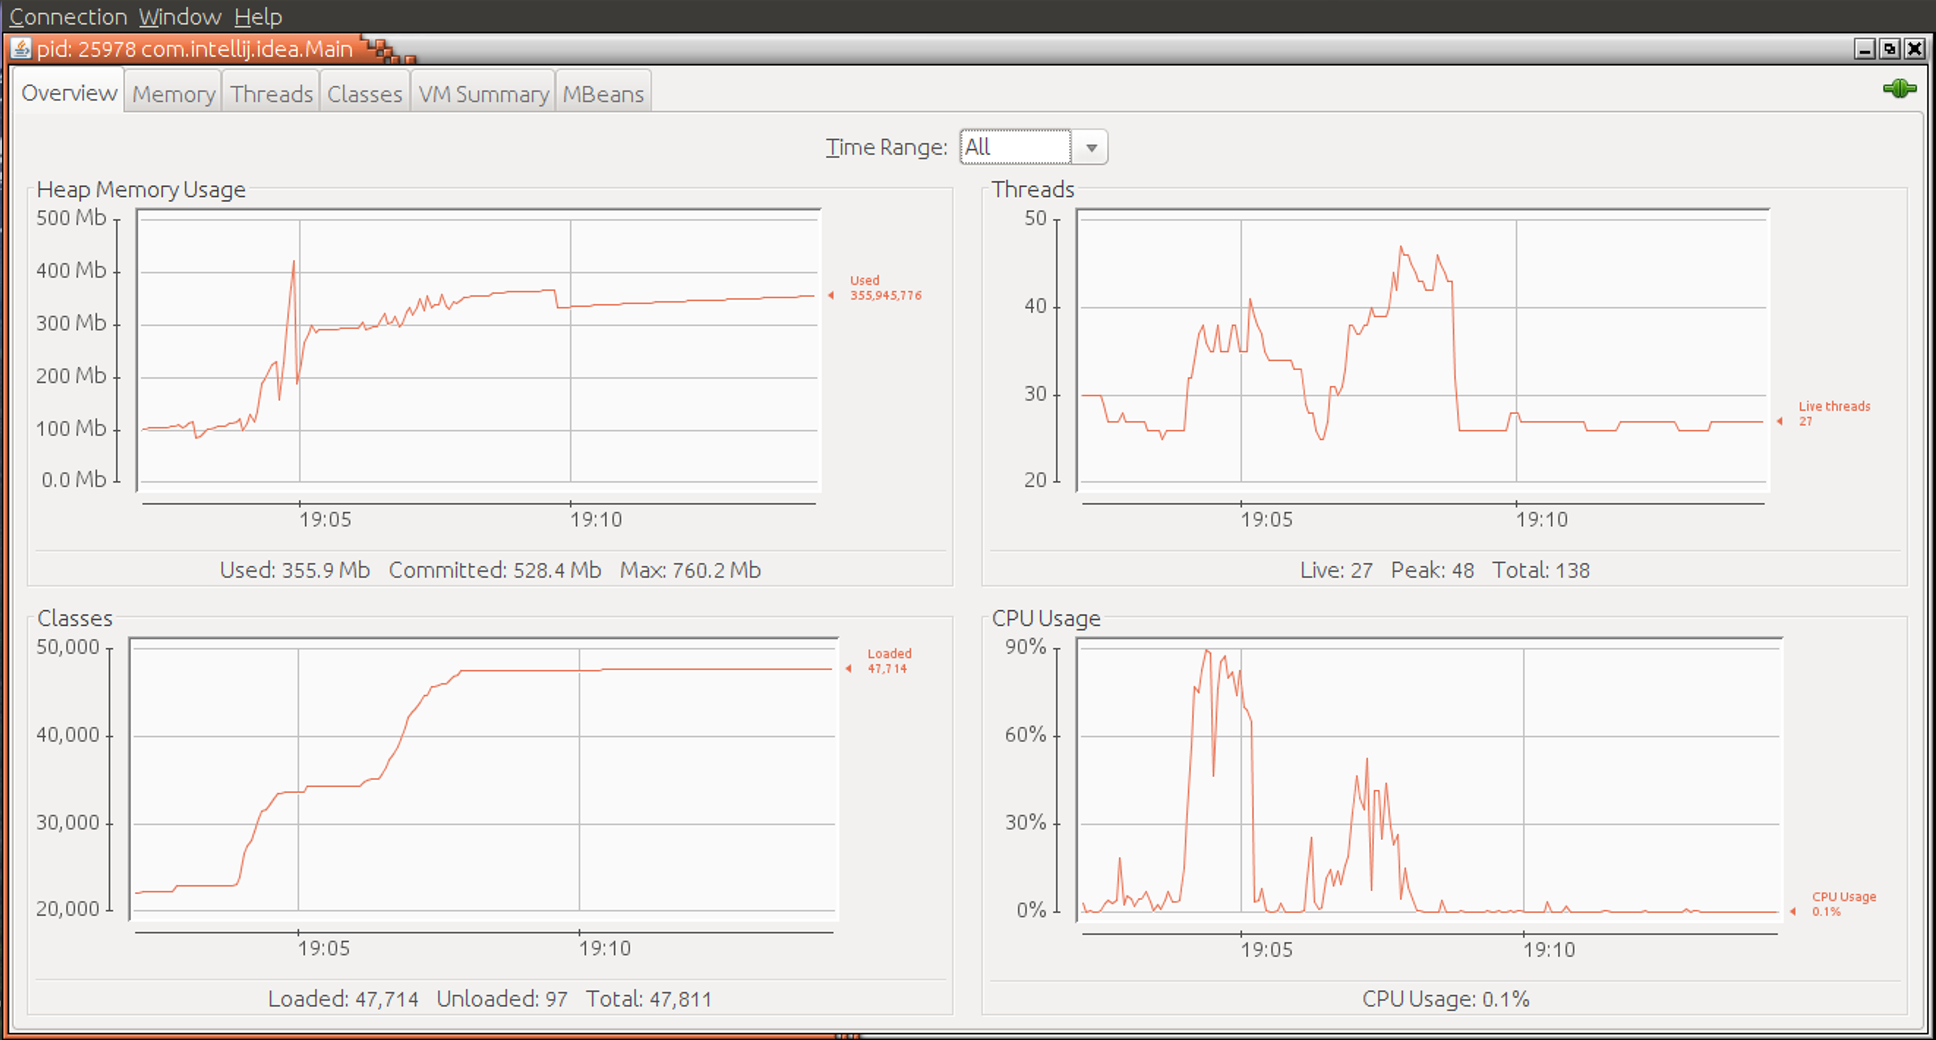
\includegraphics[width=13cm]{fig/jconsole.png}
	\caption{A JDK 8 JConsole tool main window. It shows use of resources, another tabs contain more detailed information and a facility to manage object called a MBeans.}
	\label{jconsole}
\end{figure}

\section{Automatic optimization tools}\label{autoopt}

\subsection{JATT}
A JATT (JVM Auto Tuning Tool) is an open source software tool which was developed to optimize JVM. The JATT is based on the OpenTuner\footnote{"OpenTuner is a new framework for building domain-specific multi-objective program autotuners. OpenTuner supports fully customizable configuration representations, an extensible technique representation to allow for domain-specific techniques, and an easy to use interface for communicating with the tuned program." \url{http://opentuner.org/}} framework and it supports only the Linux environment. Aforementioned tool offers the Console mode and the Graphical User Interface as well. Authors highly recommend to use the console mode for more advanced work. The JATT is designed to tune especially HotSpot JVM (namely, it was tested on OpenJDK 7 update 55) but it can be modified to auto tune a different JVM.
\cite{jatt-web} \cite{jatt-web-dzone}

The \textit{JATT} is an \textbf{offline} tuning tool -- it means a tuning phase and a production phase are strictly separated. Firstly, an optimal parameter configuration that will produce best performance within specified deployment environment. Secondly, found optimal configuration is used to deploy the application. There is an opposite approach called \textbf{online} tuning which deals with finding an optimal configuration during the runtime of an application. The \textit{JATT} does not offer an online auto tuning of JVM now but it is in development. 
% TODO napsat autorum, jestli budou ve vyvoji pokracovat a podle toho dopsat
An initial phase of development indicates use of a \textit{jstat} utility\footnote{For more informations see sites \url{https://docs.oracle.com/javase/8/docs/technotes/guides/troubleshoot/tooldescr017.html} and \url{https://docs.oracle.com/javase/8/docs/technotes/tools/unix/jstat.html} for use.}. \cite{jatt}

Already stated tool is written in Python programming language\footnote{Official repository is located at \url{https://bitbucket.org/sapients/hotspottuner/}} and except for the OpenTuner it requires another packages. For a comprehensive information about requirements, installation and use see website \cite{jatt-web-medium}. There is shown simple example to auto tune 






{\color{red} Popsat JATT, applicare}


%{\color{red} In many cases, though, remember that the JVM is a small part of the overall performance picture. \cite{scott} p. 10}

%{\color{red} One particularly important case of testing a full application occurs when multiple applications are run at the same time on the same hardware. Many aspects of the JVM are	tuned by default to assume that all machine resources are available to them, and if those JVMs are tested in isolation, they will behave well. If they are tested when other applications are present (including, but not limited to, other JVMs), their performance will be quite different. \cite{scott} p. 18}

% Dotazy
% Bezi cilova aplikace izolovane nebo jsou tam i dalsi java aplikace?

%JVM je zasobnikovy pocitac
%Ergonomics - Automatic Selections and behaviour tuning 

%Java Flight Recorder
%Moznosti analyzy vykonu - vmstat jconsole, prepinace -XX:PrintGCDetails/-XX:PrintGCTimeStamps



\bibliographystyle{ieeetran}
\bibliography{bibfile}

\appendix
\chapter{Big impact options}
\begin{table}[]
	\centering
	\begin{tabular}{ll}
	\cline{1-1}
	\multicolumn{1}{|l|}{\textbf{Primitive}}                         &                                                             \\ \cline{1-1}
	\multicolumn{1}{|l|}{-d32 | -d64}                                &                                                             \\ \cline{1-1}
	\multicolumn{1}{|l|}{-server | -client}                          &                                                             \\ \cline{1-1}
	\multicolumn{1}{|l|}{-Xmixed | -Xcomp | -Xint}                   &                                                             \\ \cline{1-1}
	\multicolumn{1}{|l|}{-Xms\textless size\textgreater}              &                                                             \\ \cline{1-1}
	\multicolumn{1}{|l|}{-Xmx\textless size\textgreater}              &                                                             \\ \cline{1-1}
	\multicolumn{1}{|l|}{-Xss\textless size\textgreater}              &                                                             \\ \cline{1-1}
	\multicolumn{1}{|l|}{-XX:AggressiveOpts}                         &                                                             \\ \cline{1-1}
	\multicolumn{1}{|l|}{-XX:BackgroundCompilation}                  &                                                             \\ \cline{1-1}
	\multicolumn{1}{|l|}{-XX:CICompilerCount}                        &                                                             \\ \cline{1-1}
	\multicolumn{1}{|l|}{-XX:CICompilerCountPerCPU}                  &                                                             \\ \cline{1-1}
	\multicolumn{1}{|l|}{-XX:CompileThreshold}                       &                                                             \\ \cline{1-1}
	\multicolumn{1}{|l|}{-XX:DoEscapeAnalysis}                       &                                                             \\ \cline{1-1}
	\multicolumn{1}{|l|}{-XX:ErgoHeapSizeLimit}                      &                                                             \\ \cline{1-1}
	\multicolumn{1}{|l|}{-XX:InitialTenuringThreshold}               &                                                             \\ \cline{1-1}
	\multicolumn{1}{|l|}{-XX:Inline}                                 &                                                             \\ \cline{1-1}
	\multicolumn{1}{|l|}{-XX:MaxMetaspaceSize}                       &                                                             \\ \cline{1-1}
	\multicolumn{1}{|l|}{-XX:MaxNewSize}                             &                                                             \\ \cline{1-1}
	\multicolumn{1}{|l|}{-XX:MaxTenuringThreshold}                   &                                                             \\ \cline{1-1}
	\multicolumn{1}{|l|}{-XX:MetaspaceSize}                          &                                                             \\ \cline{1-1}
	\multicolumn{1}{|l|}{-XX:NewRatio}                               &                                                             \\ \cline{1-1}
	\multicolumn{1}{|l|}{-XX:NewSize}                                &                                                             \\ \cline{1-1}
	\multicolumn{1}{|l|}{-XX:SoftRefLRUPolicyMSPerMB}                &                                                             \\ \cline{1-1}
	\multicolumn{1}{|l|}{-XX:SurvivorRatio}                          &                                                             \\ \cline{1-1}
	\multicolumn{1}{|l|}{-XX:ThreadStackSize}                        &                                                             \\ \cline{1-1}
	\multicolumn{1}{|l|}{-XX:UseBiasedLocking}                       &                                                             \\ \cline{1-1}
	\multicolumn{1}{|l|}{-XX:UseGCOverheadLimit}                     &                                                             \\ \cline{1-1}
	\multicolumn{1}{|l|}{-XX:UseParallelOldGC}                       &                                                             \\ \cline{1-1}
	\multicolumn{1}{|l|}{-XX:UseSerialGC}                            &                                                             \\ \cline{1-1}
	\end{tabular}
	\caption{The big impact primitive options. It's possible to use any option without enabling the other one. These options subject subsequent optimization.}
	\label{bigimpactprimitive}
\end{table}
	
	
	

\begin{table}[]
	\centering
	\begin{tabular}{|l|l|}
		\hline
		\multicolumn{2}{|l|}{\textbf{Complex}}                                              \\ \hline
		-server                                    & -XX:TieredCompilation                  \\ \hline
		\multirow{4}{*}{-XX:UseParallelGC}         & -XX:InitialSurvivorRatio               \\ \cline{2-2} 
		& -XX:MinSurvivorRatio                   \\ \cline{2-2} 
		& -XX:TargetSurvivorRatio                \\ \cline{2-2} 
		& -XX:GCTimeRatio                        \\ \hline
		\multirow{4}{*}{-XX:UseConcMarkSweepGC}    & -XX:CMSInitiatingOccupancyFraction     \\ \cline{2-2} 
		& -XX:UseCMSInitiatingOccupancyOnly      \\ \cline{2-2} 
		& -XX:ConcGCThreads                      \\ \cline{2-2} 
		& -XX:CMSClassUnloadingEnabled           \\ \hline
		\multirow{2}{*}{-XX:UseAdaptiveSizePolicy} & -XX:UseAdaptiveSizePolicyFootprintGoal \\ \cline{2-2} 
		& -XX:UseAdaptiveSizePolicyWithSystemGC  \\ \hline
		\multirow{3}{*}{-XX:UseG1GC}               & -XX:ConcGCThreads                      \\ \cline{2-2} 
		& -XX:UseStringDeduplication             \\ \cline{2-2} 
		& -XX:G1MixedGCLiveThresholdPercent      \\ \hline
		All GC except Serial GC                    & -XX:ParallelGCThreads                  \\ \hline
	\end{tabular}
	\caption{The big impact complex options. To use the option from the right column it's necessary to enable the  option from the left column. These options subject subsequent optimization.}
	\label{bigimpactcomplex}
\end{table}		


\end{document}
